% thông tin giới thiệu
Trong chương này sẽ trình bày về cơ sở lý thuyết của thuật toán học máy tăng
cường sâu \ac{drl}, thuật toán nhận diện vật thể \ac{yl} và môi trường giả lập giao
thông đô thị \ac{sumo}.

\section{Hệ thống điều khiển giao thông thích ứng - \ac{atsc}}
\subsection{Khái niệm và thông tin tổng quan}
Các phương pháp điều khiển tín hiệu giao thông tự điều chỉnh theo điều kiện giao
thông được gọi chung là hệ thống điều khiển giao thông thích ứng (\ac{atsc}) \cite{Shams2023}.
Không giống như các hệ thống điều khiển theo thời gian cố định hoạt động dựa
trên các kế hoạch được lập trình sẵn, \ac{atsc} sử dụng dữ liệu thời gian thực
từ các cảm biến (ví dụ: vòng từ, camera, radar) để liên tục tối ưu hóa các thông
số của đèn tín hiệu. Mục tiêu chính của \ac{atsc} là cải thiện hiệu quả của mạng
lưới giao thông bằng cách giảm thiểu độ trễ, số lần dừng, mức tiêu thụ nhiên liệu
và khí thải \cite{Stevanovic2010}.

Các hệ thống \ac{atsc} có thể được phân loại dựa trên nhiều tiêu chí khác nhau, chẳng
hạn như cấu trúc điều khiển (tập trung, phân cấp, phân tán), phương pháp ra
quyết định (dựa trên luật, tối ưu hóa), và cơ chế phối hợp giữa các nút giao
\cite{Shams2023}. Sự phát triển của \ac{atsc} đã trải qua nhiều thế hệ, từ các hệ
thống lựa chọn kế hoạch tín hiệu có sẵn (Thế hệ 1) đến các hệ thống điều chỉnh kế
hoạch tín hiệu (Thế hệ 2), và các hệ thống điều khiển thời gian thực không dựa
trên chu kỳ cố định (Thế hệ 3).
\newpage
\subsection{Nguyên lý hoạt động}
Về cơ bản, \ac{atsc} hoạt động theo một vòng lặp gồm ba bước chính được minh họa trong 
% Hình \ref{fig:atsc_operation}:

% \begin{figure*}[!htp]
%     \centering
%     \includegraphics[width=0.8\textwidth]{figures/atsc_operation_diagram.png}
%     \caption{Sơ đồ nguyên lý hoạt động của hệ thống ATSC}
%     \label{fig:atsc_operation}
% \end{figure*}

\begin{enumerate}
    \item \textbf{Thu thập dữ liệu (Data Collection):} Các cảm biến được lắp đặt
        tại các vị trí chiến lược trên mạng lưới đường phố để thu thập dữ liệu
        giao thông theo thời gian thực như lưu lượng, mật độ, tốc độ và chiều
        dài hàng chờ của xe. Công nghệ xe kết nối (Connected Vehicle - CV) cũng hứa
        hẹn cung cấp nguồn dữ liệu chi tiết và chính xác hơn cho các hệ thống \ac{atsc}
        trong tương lai \cite{Wang2018}.

    \item \textbf{Xử lý và tối ưu hóa (Processing and Optimization):} Dữ liệu
        thu thập được sẽ được truyền đến bộ điều khiển. Tại đây, các thuật toán
        phức tạp sẽ phân tích dữ liệu, dự báo các điều kiện giao thông sắp tới và
        tính toán các thông số thời gian tín hiệu tối ưu (thời gian chu kỳ, phân
        chia pha, độ lệch) cho một hoặc một nhóm các nút giao. Quá trình tối ưu
        hóa này có thể dựa trên các mô hình toán học, các phương pháp phỏng đoán
        (heuristics), hoặc các kỹ thuật trí tuệ nhân tạo như học tăng cường
        \cite{Wei2019}.

    \item \textbf{Thực thi điều khiển (Control Implementation):} Các thông số
        thời gian tín hiệu mới được tính toán sẽ được gửi đến các bộ điều khiển
        đèn tín hiệu tại các nút giao để thực thi. Vòng lặp này được lặp lại liên
        tục, cho phép hệ thống liên tục "thích ứng" với sự thay đổi của luồng
        giao thông.
\end{enumerate}

\subsection{Các hệ thống tiêu biểu đã được triển khai}
Trên thế giới, có nhiều hệ thống \ac{atsc} đã được thương mại hóa và triển khai
rộng rãi. Hai trong số những hệ thống nổi tiếng và có ảnh hưởng nhất là SCATS và
SCOOT.

\subsubsection{Sydney Coordinated Adaptive Traffic System (SCATS)}
Được phát triển tại Sydney, Úc vào những năm 1970, SCATS là một hệ thống quản lý
giao thông thông minh hoạt động theo kiến trúc điều khiển phân cấp và có khả năng
lựa chọn kế hoạch tín hiệu \cite{Sims1980}.
\begin{itemize}
    \item \textbf{Nguyên lý:} Hoạt động của SCATS dựa trên việc đo lường "mức độ
        bão hòa" (degree of saturation) tại các vạch dừng của nút giao thông
        thông qua các vòng từ cảm ứng. Dữ liệu này được các bộ điều khiển cục bộ
        sử dụng để thực hiện các điều chỉnh nhỏ trong thời gian thực cho pha đèn.
        Ở cấp độ cao hơn, các máy tính khu vực sẽ thu thập dữ liệu từ nhiều nút giao
        để lựa chọn một trong số các kế hoạch phối hợp (bao gồm thời gian chu kỳ,
        phân chia pha, và độ lệch) đã được các kỹ sư giao thông xây dựng trước và
        lưu trong thư viện.

    \item \textbf{Đặc điểm:} SCATS không tự tạo ra các kế hoạch thời gian hoàn
        toàn mới mà lựa chọn kế hoạch phù hợp nhất từ một thư viện định sẵn và
        tinh chỉnh nó. Điều này giúp hệ thống hoạt động ổn định và có khả năng tự
        động điều chỉnh mà không cần nhiều sự can thiệp thủ công, qua đó giảm
        chi phí vận hành.
\end{itemize}

\subsubsection{Split Cycle Offset Optimisation Technique (SCOOT)}
SCOOT được phát triển tại Vương quốc Anh cùng thời với SCATS, là một hệ thống
tối ưu hóa thời gian thực, tập trung \cite{Hunt1981}.
\begin{itemize}
    \item \textbf{Nguyên lý:} Khác với SCATS, SCOOT không dựa vào các kế hoạch có
        sẵn. Thay vào đó, nó sử dụng các mô hình dự báo luồng giao thông (dựa
        trên dữ liệu từ các cảm biến đặt ở đầu nút giao) để dự đoán mô hình đến của
        xe tại các nút giao. Dựa trên các dự báo này, một máy tính trung tâm sẽ liên
        tục thực hiện những điều chỉnh nhỏ và thường xuyên (vài giây một lần) đối
        với thời gian chu kỳ, phân chia pha và độ lệch.

    \item \textbf{Đặc điểm:} Mục tiêu của SCOOT là tối ưu hóa một "chỉ số hiệu suất"
        (Performance Index), thường là một hàm kết hợp giữa tổng độ trễ và số lần
        dừng xe trong toàn mạng lưới. Bằng cách liên tục thực hiện các điều
        chỉnh nhỏ, SCOOT có khả năng thích ứng rất linh hoạt với những biến động
        của giao thông, ngay cả trong cùng một chu kỳ tín hiệu.
\end{itemize}

\section{Học tăng cường và Học tăng cường sâu}
\subsection{Học tăng cường (Reinforcement Learning)}
\subsubsection{Khái niệm cơ bản}
Học tăng cường (Reinforcement Learning - \ac{rl}) là một lĩnh vực của học máy, tập
trung vào việc huấn luyện một tác nhân (agent) cách ra quyết định trong một môi trường
(environment) để tối đa hóa một tín hiệu phần thưởng tích lũy. Khác với các mô
hình học máy khác, \ac{rl} học thông qua quá trình thử và sai (trial and error),
tương tự như cách con người và động vật học từ kinh nghiệm \cite{Sutton2018}.
Tác nhân không được chỉ dẫn hành động nào là đúng, mà phải tự khám phá ra chiến lược
(policy) tốt nhất bằng cách thực hiện hành động và quan sát kết quả.

\subsubsection{Các thành phần chính}
Một bài toán \ac{rl} điển hình được định nghĩa bởi các thành phần cốt lõi sau:
\begin{itemize}
    \item \textbf{Tác nhân (Agent):} Là thực thể ra quyết định và thực hiện hành
        động. Trong bối cảnh điều khiển giao thông, tác nhân có thể là bộ điều
        khiển đèn tín hiệu.

    \item \textbf{Môi trường (Environment):} Là thế giới mà tác nhân tương tác. Đối
        với bài toán giao thông, môi trường là mạng lưới giao thông, bao gồm các
        nút giao, làn đường và phương tiện.

    \item \textbf{Trạng thái (State - $s$):} Là một mô tả cụ thể về môi trường
        tại một thời điểm nhất định. Ví dụ: số lượng xe đang chờ ở mỗi làn đường,
        thời gian đèn xanh hiện tại.

    \item \textbf{Hành động (Action - $a$):} Là một lựa chọn mà tác nhân có thể
        thực hiện. Ví dụ: giữ nguyên pha đèn hiện tại, chuyển sang pha đèn tiếp theo.

    \item \textbf{Phần thưởng (Reward - $r$):} Là tín hiệu phản hồi từ môi
        trường sau khi tác nhân thực hiện một hành động. Phần thưởng cho biết hành
        động đó tốt hay xấu. Ví dụ: phần thưởng có thể là giá trị âm của tổng thời
        gian chờ của các xe, mục tiêu là tối đa hóa phần thưởng (tức giảm thiểu thời
        gian chờ).
\end{itemize}

\subsubsection{Vòng lặp học tập}
Reinforcement Learning hoạt động dựa trên một quy trình tương tác liên tục giữa agent và môi trường. Hình \ref{fig:RL-components} minh họa các thành phần và luồng thông tin trong vòng lặp học tập cơ bản.

\begin{figure*}[!htp]
    \centering
    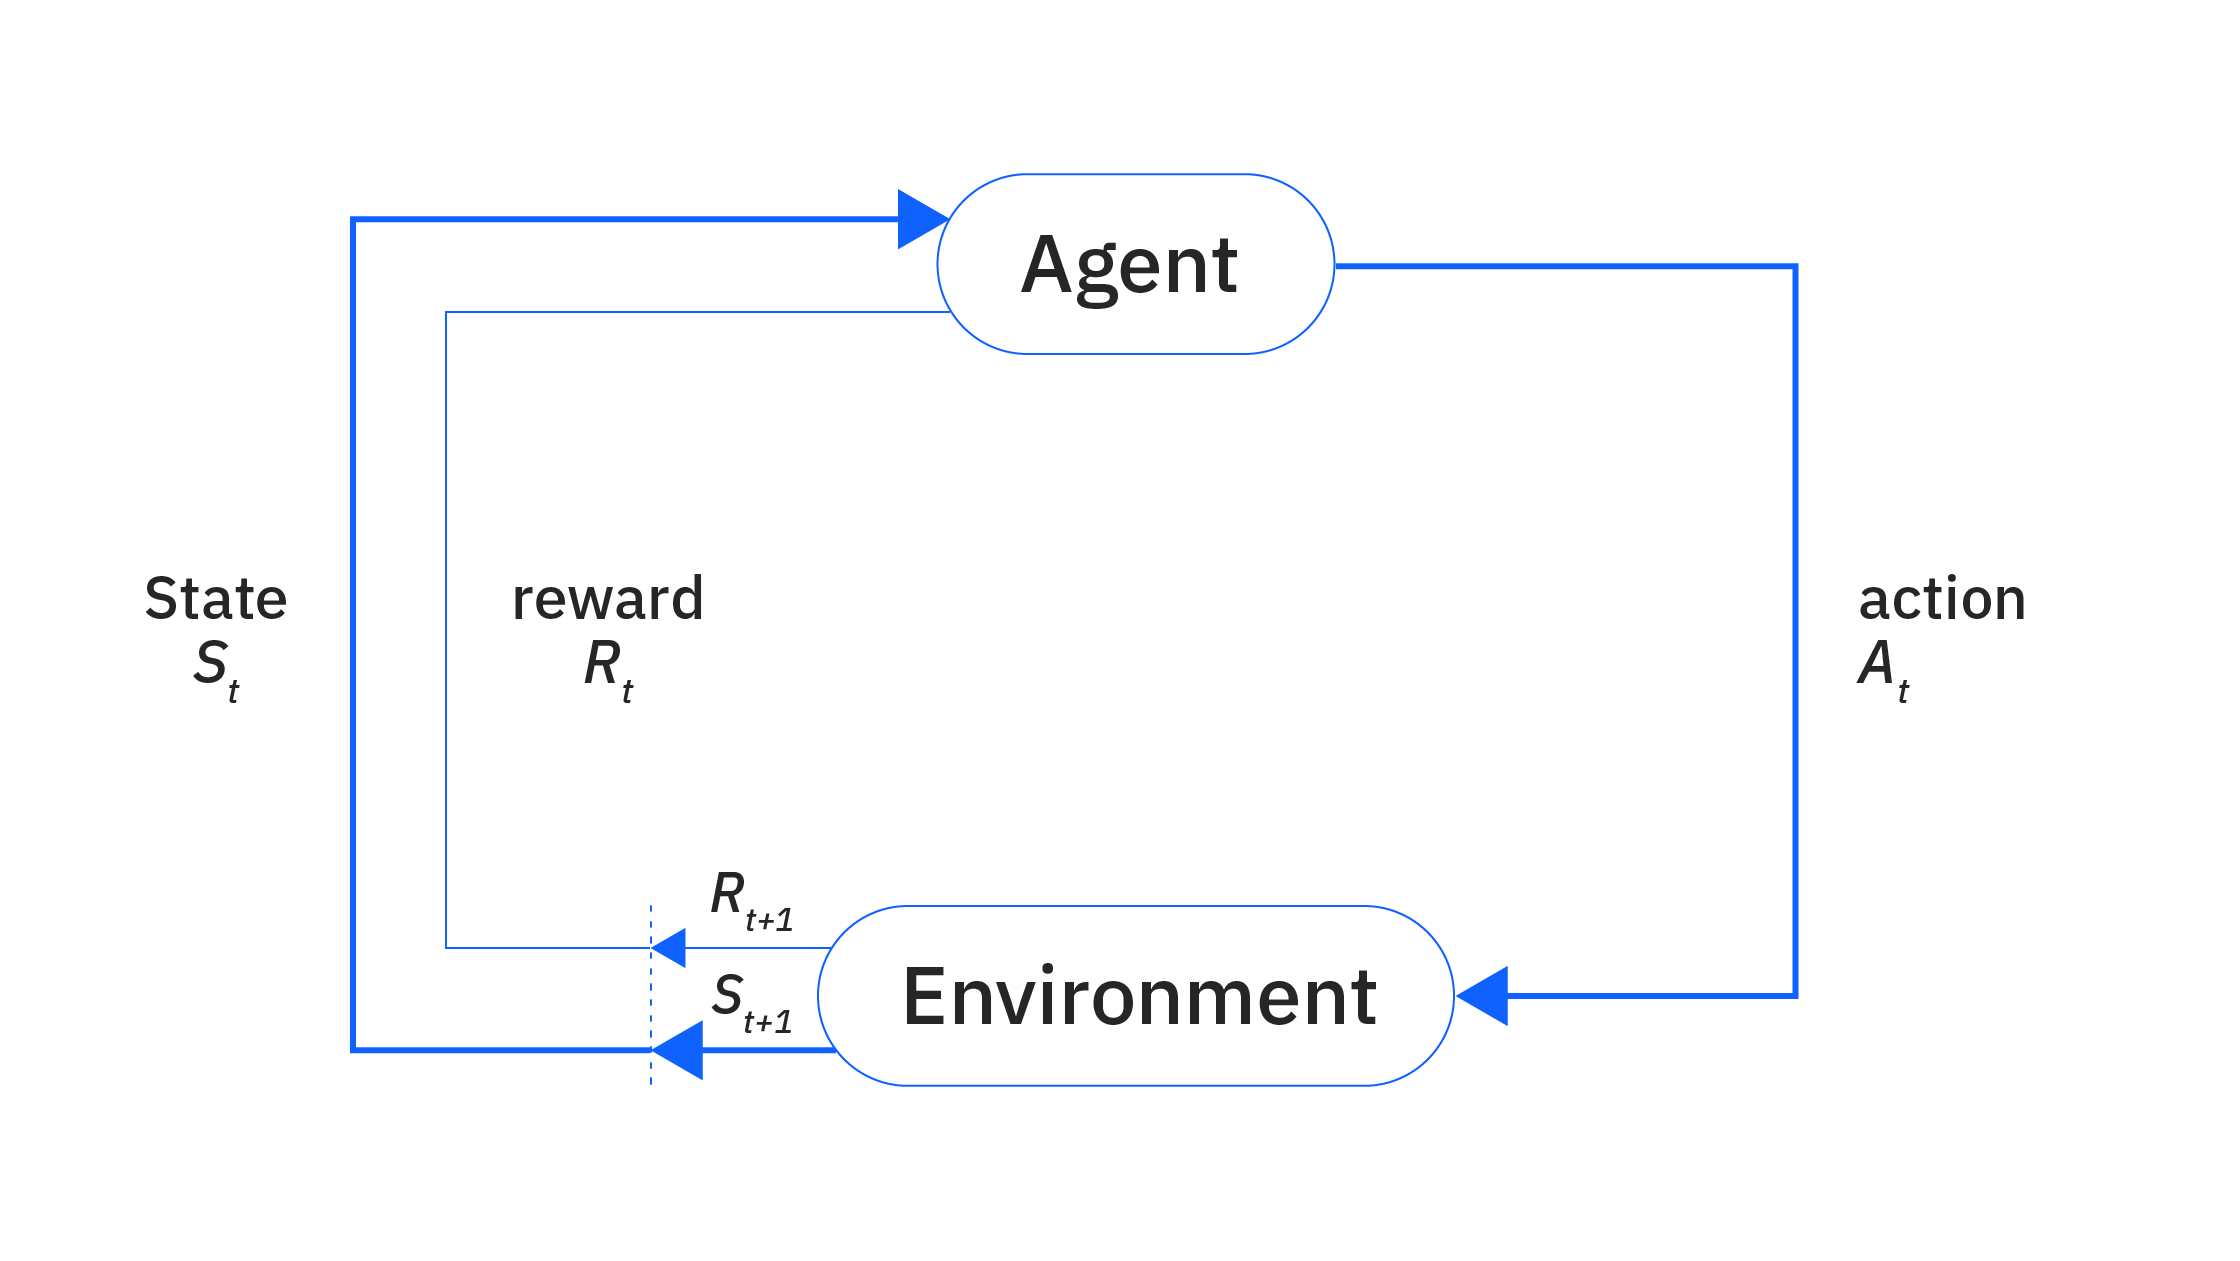
\includegraphics[width=0.8\textwidth]{img/RL_components.png}
    \caption{Vòng lặp học tập của Reinforcement Learning \cite{IBM2024}}
    \label{fig:RL-components}
\end{figure*}
Quá trình học của \ac{rl} diễn ra theo một vòng lặp liên tục:

\begin{enumerate}
    \item Tác nhân quan sát trạng thái hiện tại $s_{t}$ của môi trường.

    \item Dựa trên trạng thái $s_{t}$, tác nhân chọn một hành động $a_{t}$.

    \item Tác nhân thực hiện hành động $a_{t}$.

    \item Môi trường chuyển sang trạng thái mới $s_{t+1}$ và trả về một phần thưởng        $r_{t+1}$ cho tác nhân.

    \item Tác nhân sử dụng thông tin về phần thưởng và trạng thái mới để cập nhật kiến thức của mình, nhằm đưa ra quyết định tốt hơn trong tương lai.
\end{enumerate}

\subsubsection{Đặc điểm khác biệt so với các phương pháp học máy khác}
\ac{rl} khác biệt cơ bản với hai nhánh còn lại của học máy:
\begin{itemize}
    \item \textbf{So với Học có giám sát (Supervised Learning):} Học có giám sát
        học từ một tập dữ liệu đã được gán nhãn sẵn. Ngược lại, trong \ac{rl},
        không có "câu trả lời đúng" cho mỗi trạng thái; tác nhân phải tự tìm ra hành
        động tối ưu. Tín hiệu phản hồi (phần thưởng) cũng có thể bị trễ, không nhất
        thiết phải có ngay sau mỗi hành động.

    \item \textbf{So với Học không giám sát (Unsupervised Learning):} Học không
        giám sát tìm kiếm cấu trúc tiềm ẩn trong dữ liệu không có nhãn. \ac{rl}
        khác ở chỗ nó có một mục tiêu rõ ràng là tối đa hóa phần thưởng, trong khi
        học không giám sát thường không có một mục tiêu tối ưu hóa cụ thể.
\end{itemize}

\subsubsection{Các thuật toán cơ bản}
Các thuật toán \ac{rl} có thể được phân loại thành các nhóm chính như dựa trên giá
trị (Value-Based), dựa trên chiến lược (Policy-Based), và lai ghép Tác nhân-Phê bình
(Actor-Critic).

\subsection{Q-Learning}
\subsubsection{Định nghĩa Q-Learning}
Q-Learning là một thuật toán \ac{rl} kinh điển, thuộc nhóm dựa trên giá trị và không
cần mô hình (model-free). "Không cần mô hình" có nghĩa là tác nhân không cần
hiểu đầy đủ về các quy tắc vận hành của môi trường. Thay vào đó, nó học trực
tiếp từ kinh nghiệm tương tác.

\subsubsection{Hàm giá trị Q}
Trọng tâm của Q-Learning là học một hàm giá trị hành động, gọi là hàm Q-function,
ký hiệu là $Q(s, a)$. Hàm này ước tính tổng phần thưởng chiết khấu trong tương lai
(còn gọi là giá trị Q) mà tác nhân sẽ nhận được nếu nó thực hiện hành động $a$ từ
trạng thái $s$, và sau đó tuân theo chiến lược tối ưu.

\subsubsection{Cơ chế cập nhật giá trị Q và Phương trình Bellman}
Trong các bài toán có không gian trạng thái và hành động nhỏ, hàm Q có thể được lưu
trong một bảng (Q-table). Các giá trị trong bảng được khởi tạo ngẫu nhiên và cập
nhật lặp đi lặp lại bằng phương trình tối ưu Bellman:
\begin{equation}
    Q(s_{t}, a_{t}) \leftarrow Q(s_{t}, a_{t}) + \alpha [r_{t+1}+ \gamma \max_{a}
    Q(s_{t+1}, a) - Q(s_{t}, a_{t})]
\end{equation}
Trong đó, $(r_{t+1}+ \gamma \max_{a}Q(s_{t+1}, a))$ là "giá trị mục tiêu" (target)
mà $Q(s_{t}, a_{t})$ đang cố gắng học.

\subsubsection{Ưu và nhược điểm}
\begin{itemize}
    \item \textbf{Ưu điểm:} Q-Learning đơn giản, dễ triển khai và được chứng minh
        là sẽ hội tụ đến chiến lược tối ưu nếu mỗi cặp (trạng thái, hành động)
        được ghé thăm đủ nhiều lần.

    \item \textbf{Nhược điểm:} Hạn chế lớn nhất của Q-Learning là "lời nguyền của
        chiều dữ liệu". Khi số lượng trạng thái hoặc hành động quá lớn, Q-table
        sẽ trở nên cồng kềnh, đòi hỏi bộ nhớ khổng lồ và thời gian học rất lâu.
        Nó cũng không thể xử lý các không gian trạng thái hoặc hành động liên
        tục.
\end{itemize}

\subsection{Học tăng cường sâu (Deep Reinforcement Learning)}
\subsubsection{Tích hợp mạng nơ-ron với RL}
Học tăng cường sâu (\ac{drl}) ra đời để giải quyết bài toán về chiều dữ liệu của
\ac{rl} truyền thống. Thay vì dùng Q-table, \ac{drl} sử dụng một mạng nơ-ron sâu
(Deep Neural Network - \ac{dnn}) để xấp xỉ hàm giá trị (như Q-function) hoặc trực
tiếp hàm chiến lược \cite{Mnih2015}.

\subsubsection{Kiến trúc mạng nơ-ron và ưu điểm}
Mạng nơ-ron nhận đầu vào là trạng thái của môi trường và đưa ra đầu ra là giá trị
Q cho mỗi hành động hoặc một phân phối xác suất trên các hành động. Ưu điểm
chính của việc tích hợp này là:
\begin{itemize}
    \item \textbf{Khả năng khái quát hóa:} Mạng nơ-ron có thể đưa ra dự đoán cho
        cả những trạng thái chưa từng gặp, dựa trên sự tương đồng với các trạng thái
        đã học.

    \item \textbf{Xử lý đầu vào phức tạp:} \ac{drl} có thể học trực tiếp từ dữ liệu
        thô, có chiều dữ liệu cao như hình ảnh, mà không cần trích xuất đặc trưng
        thủ công.
\end{itemize}

\subsubsection{Các framework phổ biến}
Việc triển khai các thuật toán \ac{drl} được hỗ trợ bởi nhiều framework mạnh mẽ như
TensorFlow, PyTorch, và các thư viện chuyên dụng như Stable Baselines3, RLlib.

\subsection{Deep Q-Learning}
\subsubsection{Nguyên lý hoạt động}
Deep Q-Learning (hay \ac{dqn}) là thuật toán kết hợp trực tiếp ý tưởng của Q-Learning
với mạng nơ-ron sâu \ac{dnn}. Nguyên lý hoạt động của nó là biến bài toán tìm giá
trị Q tối ưu thành một bài toán học có giám sát.

Mạng nơ-ron, được gọi là Q-network, sẽ nhận đầu vào là trạng thái $s$ và đầu ra là
một vector các giá trị Q, mỗi giá trị tương ứng với một hành động có thể thực
hiện $Q(s, \cdot; \theta)$, trong đó $\theta$ là các trọng số của mạng. Quá
trình huấn luyện nhằm điều chỉnh các trọng số $\theta$ sao cho giá trị
$Q(s, a; \theta)$ do mạng dự đoán ngày càng gần với giá trị mục tiêu $y$:
\begin{equation}
    y = r + \gamma \max_{a'}Q(s', a'; \theta)
\end{equation}
Sự chênh lệch giữa giá trị dự đoán và giá trị mục tiêu được đo bằng một hàm mất mát,
thường là Sai số bình phương trung bình (Mean Squared Error - MSE). Sau đó,
thuật toán lan truyền ngược (backpropagation) và hạ gradient (gradient descent)
được sử dụng để cập nhật các trọng số $\theta$ nhằm tối thiểu hóa hàm mất mát
này.

\subsubsection{Kiến trúc mạng và các kỹ thuật ổn định hóa}
Việc thay thế Q-table bằng mạng nơ-ron một cách trực tiếp có thể gây ra sự mất
ổn định trong huấn luyện. \ac{dqn} giới thiệu hai kỹ thuật để giải quyết
vấn đề này:
\begin{itemize}
    \item \textbf{Experience Replay (Bộ nhớ tái hiện kinh nghiệm):} Tác nhân lưu
        trữ các kinh nghiệm $(s, a, r, s')$ vào một bộ nhớ đệm. Thay vì học từ kinh
        nghiệm gần nhất, nó lấy một lô dữ liệu nhỏ ngẫu nhiên từ bộ nhớ để huấn
        luyện. Điều này giúp phá vỡ sự tương quan giữa các mẫu dữ liệu liên tiếp,
        làm cho quá trình học ổn định hơn.

    \item \textbf{Target Network (Mạng mục tiêu):} \ac{dqn} sử dụng hai mạng:
        một mạng chính được cập nhật liên tục và một mạng mục tiêu được giữ cố
        định. Mạng mục tiêu được dùng để tính toán giá trị Q mục tiêu, tạo ra
        một "đích đến" ổn định cho mạng chính học theo. Trọng số của mạng mục tiêu
        được sao chép từ mạng chính sau một số bước nhất định.
\end{itemize}

\subsubsection{Các biến thể và phát triển}
Kể từ khi ra đời, \ac{dqn} đã có nhiều biến thể cải tiến quan trọng, ví dụ:
\begin{itemize}
    \item \textbf{Double DQN:} Giảm thiểu việc đánh giá quá cao các giá trị Q, giúp
        quá trình học ổn định và chính xác hơn.

    \item \textbf{Dueling DQN:} Sử dụng một kiến trúc mạng đặc biệt, tách biệt việc
        ước tính giá trị của trạng thái (state value) và lợi thế của từng hành động
        (action advantage), giúp học hiệu quả hơn.
\end{itemize}

\section{Thuật toán nhận diện vật thể YOLO}
\subsection{Tổng quan về YOLO}
YOLO (You Only Look Once) là một thuật toán phát hiện đối tượng theo thời gian thực,
được giới thiệu lần đầu tiên vào năm 2015. Khác với các phương pháp phát hiện
đối tượng truyền thống sử dụng phương pháp hai giai đoạn (two-stage detection), YOLO
xử lý phát hiện đối tượng như một vấn đề hồi quy đơn lẻ, dự đoán các hộp giới
hạn và xác suất lớp trực tiếp từ hình ảnh đầy đủ trong một lần đánh giá
\cite{Redmon2016}. Phương pháp này giúp YOLO đạt được tốc độ xử lý nhanh hơn đáng
kể so với các phương pháp trước đó.

\subsection{Nguyên lý hoạt động}
YOLO áp dụng cách tiếp cận khác biệt trong bài toán phát hiện đối tượng so với các phương pháp truyền thống, khi xử lý toàn bộ hình ảnh chỉ trong một lần duy nhất thay vì chia nhỏ và xử lý trên từng vùng. Hình \ref{fig:yolo_architecture} minh họa cách thức hoạt động của thuật toán này.

\begin{figure}[!htp]
    \centering
    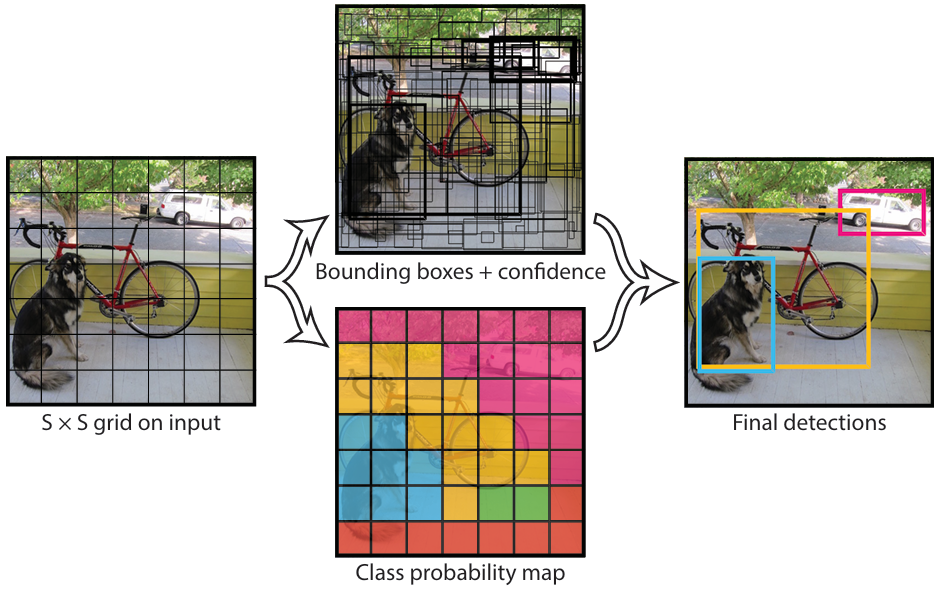
\includegraphics[width=0.6\textwidth]{img/yolo_1}
    \caption{Nguyên lý hoạt động của YOLO}
    \label{fig:yolo_architecture}
\end{figure}

Cụ thể, thuật toán chia hình ảnh đầu vào thành một lưới $S \times S$ cells. Mỗi cell chịu
trách nhiệm dự đoán các đối tượng có tâm nằm trong nó. Mỗi cell dự đoán:
\begin{itemize}
    \item $B$ bounding boxes và độ tin cậy (confidence scores) cho mỗi box

    \item $C$ xác suất có điều kiện của các lớp đối tượng
\end{itemize}

Mỗi bounding box bao gồm 5 thành phần dự đoán:
\begin{equation}
    (x, y, w, h, confidence)
\end{equation}
Trong đó:
\begin{itemize}
    \item $(x, y)$ là tọa độ tâm của box, tương đối so với ranh giới của cell

    \item $(w, h)$ là chiều rộng và chiều cao của box, tương đối so với kích
        thước toàn bộ hình ảnh

    \item $confidence$ phản ánh độ tin cậy của box và độ chính xác của vị trí box
\end{itemize}

\subsection{Quá trình dự đoán}
Quá trình dự đoán của YOLO bao gồm các bước chính:
\begin{enumerate}
    \item \textbf{Xử lý đầu vào:} Hình ảnh được resize về kích thước cố định và
        chia thành lưới $S \times S$.

    \item \textbf{Trích xuất đặc trưng:} Sử dụng mạng \ac{cnn} để trích xuất các
        đặc trưng từ hình ảnh.

    \item \textbf{Dự đoán:} Mỗi cell dự đoán $B$ bounding boxes và xác suất lớp.

    \item \textbf{Lọc kết quả:} Áp dụng ngưỡng confidence và Non-Maximum
        Suppression (NMS) để loại bỏ các dự đoán trùng lặp.
\end{enumerate}

\section{Môi trường mô phỏng giao thông đô thị SUMO}
\ac{sumo}~\footnote{SUMO - Simulation of Urban MObility: \url{https://www.eclipse.org/sumo/}} (Simulation of Urban MObility) là một bộ phần mềm giả lập giao thông vi
mô, mã nguồn mở, và đa nền tảng, được phát triển bởi Trung tâm Hàng không Vũ trụ
Đức. Mục tiêu chính của \ac{sumo} là cung cấp một công cụ mạnh mẽ và linh hoạt
để nghiên cứu các hệ thống giao thông, cho phép các nhà nghiên cứu, kỹ sư và nhà
hoạch định chính sách mô hình hóa, phân tích và đánh giá các kịch bản giao thông
khác nhau mà không cần triển khai trong thế giới thực.

Là một công cụ giả lập vi mô, \ac{sumo} mô hình hóa từng phương tiện riêng lẻ trong
mạng lưới. Mỗi phương tiện có các thuộc tính và hành vi riêng (ví dụ: mô hình
bám đuôi xe, mô hình chuyển làn), và sự tương tác của chúng tạo nên các hiện tượng
giao thông vĩ mô như tắc nghẽn. Điều này làm cho \ac{sumo} trở thành một môi trường
lý tưởng để thử nghiệm các thuật toán điều khiển giao thông thông minh, đặc biệt
là các phương pháp dựa trên \ac{drl}, nơi tác nhân cần một môi trường chi tiết
để học hỏi và tương tác.

\subsection{Các thành phần và kiến trúc cốt lõi}
Một kịch bản giả lập trong \ac{sumo} thường bao gồm ba loại tệp chính:
\begin{itemize}
    \item Mạng lưới giao thông

    \item Nhu cầu giao thông

    \item Cấu hình giả lập
\end{itemize}

\subsubsection{Mạng lưới giao thông (Network)}
Mạng lưới định nghĩa cơ sở hạ tầng đường bộ, được lưu trong tệp có phần mở rộng
\texttt{.net.xml}. Nó bao gồm:
\begin{itemize}
    \item \textbf{Nodes (Nút):} Đại diện cho các nút giao thông hoặc các điểm
        cuối của một con đường.

    \item \textbf{Edges (Cạnh):} Đại diện cho các đoạn đường kết nối các nút. Mỗi
        cạnh có các thuộc tính như số làn, giới hạn tốc độ, và quyền ưu tiên.

    \item \textbf{Traffic Lights (Đèn tín hiệu):} Logic điều khiển tại các nút
        giao, bao gồm các pha và thời gian của chúng.
\end{itemize}
\ac{sumo} cung cấp công cụ \texttt{netedit}, một trình soạn thảo đồ họa, cho phép
người dùng dễ dàng tạo và chỉnh sửa các mạng lưới này. Ngoài ra, \ac{sumo} cũng
có thể nhập mạng lưới từ các nguồn dữ liệu thực tế như OpenStreetMap.

\subsubsection{Nhu cầu giao thông (Demand)}
Nhu cầu giao thông mô tả các phương tiện và hành trình của chúng trong mạng lưới,
thường được định nghĩa trong tệp \texttt{.rou.xml}. Các thành phần chính bao gồm:
\begin{itemize}
    \item \textbf{Vehicle Types (Loại phương tiện):} Định nghĩa các đặc tính vật
        lý và hành vi của phương tiện, chẳng hạn như chiều dài, gia tốc tối đa, giảm
        tốc, và cả mô hình hành vi của người lái xe (ví dụ: mức độ "hoàn hảo"
        của tài xế).

    \item \textbf{Routes (Tuyến đường):} Là một chuỗi các cạnh mà một phương
        tiện sẽ đi qua.

    \item \textbf{Flows (Luồng phương tiện):} Cho phép định nghĩa một lượng lớn
        phương tiện được tạo ra theo thời gian, thay vì phải định nghĩa từng chiếc
        xe một. Điều này rất hữu ích để mô phỏng các kịch bản giao thông thực tế
        với lưu lượng lớn.
\end{itemize}

\subsubsection{Cấu hình giả lập (Configuration)}
Tệp cấu hình, thường có đuôi \texttt{.sumocfg}, là tệp chính để chạy một kịch
bản giả lập. Nó chỉ định các tệp đầu vào cần thiết (như tệp mạng lưới và tệp nhu
cầu), thời gian bắt đầu và kết thúc của giả lập, và các tùy chọn đầu ra khác.

\subsection{Giao diện điều khiển TraCI (Traffic Control Interface)}
Một trong những tính năng mạnh mẽ nhất của \ac{sumo} là Giao diện Điều khiển
Giao thông (Traffic Control Interface - TraCI). Đây là một giao diện lập trình ứng
dụng (API) hoạt động dựa trên giao thức TCP, cho phép các ứng dụng bên ngoài
tương tác và điều khiển giả lập \ac{sumo} đang chạy theo thời gian thực. TraCI
mở ra khả năng kết nối \ac{sumo} với các kịch bản điều khiển phức tạp, các công
cụ phân tích dữ liệu hoặc các hệ thống phần mềm khác, chẳng hạn như một chương trình
viết bằng Python.

Quá trình tương tác thông qua TraCI hoạt động theo một vòng lặp đồng bộ giữa \ac{sumo}
và ứng dụng bên ngoài tại mỗi bước thời gian của giả lập:
\begin{enumerate}
    \item \textbf{Truy xuất dữ liệu (Data Retrieval):} Ứng dụng bên ngoài gửi
        yêu cầu và nhận về dữ liệu chi tiết từ môi trường giả lập. Các dữ liệu này
        có thể bao gồm thông tin về các đối tượng trong giả lập (ví dụ: vị trí,
        tốc độ của từng phương tiện) hoặc trạng thái của cơ sở hạ tầng (ví dụ: trạng
        thái đèn tín hiệu, số xe trên một làn đường).

    \item \textbf{Thay đổi trạng thái (State Modification):} Dựa trên dữ liệu
        thu được và logic của ứng dụng, nó có thể gửi các lệnh để thay đổi trạng
        thái của các đối tượng hoặc cơ sở hạ tầng trong giả lập. Ví dụ, một kịch
        bản có thể thay đổi tuyến đường của một phương tiện một cách linh động hoặc
        điều chỉnh chu kỳ đèn tín hiệu của một nút giao.

    \item \textbf{Tiến trình giả lập (Simulation Step):} Sau khi ứng dụng bên
        ngoài hoàn tất việc trao đổi dữ liệu, nó sẽ gửi một lệnh cho \ac{sumo}
        để tiến hành giả lập trong một khoảng thời gian ngắn (ví dụ, một giây).
        \ac{sumo} sẽ tạm dừng sau khi hoàn thành bước này và chờ lệnh tiếp theo,
        đảm bảo quá trình được đồng bộ.
\end{enumerate}
Cơ chế tương tác linh hoạt này cho phép triển khai và kiểm thử các thuật toán điều
khiển giao thông thích ứng, các chiến lược định tuyến động, hoặc thu thập dữ liệu
chi tiết cho các mục đích phân tích mà không bị giới hạn bởi các chức năng có sẵn
của \ac{sumo}. Điều này làm cho \ac{sumo} kết hợp với TraCI trở thành một nền
tảng tiêu chuẩn cho việc nghiên cứu và phát triển các hệ thống giao thông thông
minh.

\subsection{Ứng dụng của SUMO}
Nhờ vào tính linh hoạt, khả năng mở rộng và bản chất mã nguồn mở, \ac{sumo} đã được
sử dụng rộng rãi trong hàng ngàn công trình nghiên cứu khoa học trên toàn thế giới.
Dưới đây là một số ví dụ tiêu biểu về ứng dụng của \ac{sumo}:
\begin{itemize}
    \item \textbf{Đánh giá và so sánh các chiến lược điều khiển giao thông:}
        Nhiều nghiên cứu sử dụng \ac{sumo} để tạo ra một môi trường giả lập thực
        tế nhằm so sánh hiệu quả của các phương pháp điều khiển đèn tín hiệu khác
        nhau.

    \item \textbf{Huấn luyện và kiểm thử các thuật toán học tăng cường:} \ac{sumo},
        đặc biệt khi kết hợp với TraCI, đã trở thành một nền tảng tiêu chuẩn để phát
        triển các tác nhân điều khiển giao thông thông minh dựa trên học tăng cường.
        Các nhà nghiên cứu có thể tạo ra các môi trường phức tạp và đa dạng để
        huấn luyện các mô hình \ac{drl} mà không tốn chi phí và rủi ro như thử nghiệm
        trong thế giới thực.

    \item \textbf{Hiệu chỉnh mô phỏng từ dữ liệu thực tế:} Để đảm bảo tính chính
        xác của các kết quả giả lập, nhiều nghiên cứu tập trung vào việc hiệu chỉnh
        các tham số của \ac{sumo} dựa trên dữ liệu thu thập từ thế giới thực.

    \item \textbf{Nghiên cứu về mạng giao tiếp giữa các phương tiện (V2X):} \ac{sumo}
        cũng là một công cụ quan trọng trong lĩnh vực nghiên cứu mạng giao tiếp giữa
        các phương tiện (Vehicular Ad-hoc Networks - VANETs). Bằng cách tích hợp
        \ac{sumo} với các trình giả lập mạng như NS-3 hoặc OMNeT++, các nhà
        nghiên cứu có thể mô phỏng đồng thời cả hành vi di chuyển của phương
        tiện và quá trình trao đổi thông tin giữa chúng. Điều này cho phép đánh giá
        các giao thức định tuyến, các ứng dụng an toàn (ví dụ: cảnh báo va chạm)
        và các hệ thống quản lý giao thông dựa trên giao tiếp V2X trong một môi trường
        tích hợp và thực tế.
\end{itemize}